% ieee_paper.tex: CSC 6740 project report (IEEE conference format, >= 4 pages), framed as a data-mining
% pipeline: preprocessing -> analysis -> model evaluation -> interpretation.
% Build (from this folder):  latexmk -pdf ieee_paper.tex   (figures in figures/, references in *.bib)

\documentclass[conference]{IEEEtran}
\usepackage{amsmath,amssymb}
\usepackage{graphicx}
\usepackage{booktabs}
\usepackage{cite}
\usepackage{url}
\usepackage[hidelinks]{hyperref}
\graphicspath{{figures/}}
\newcommand{\dd}{\mathrm{d}}

\begin{document}

\title{Using High Frequency Imaging of Red Blood Cells to Estimate Stochastic Parameters and Transport Effects of a Fluctuating Membrane}

\author{\IEEEauthorblockN{Tommy Stell}
\IEEEauthorblockA{Georgia State University\\Atlanta, GA, USA}}

\maketitle

\begin{abstract}
A signaling molecule inside a cell diffuses in a container whose wall fluctuates, yet transport is
almost always computed with a fixed wall. We ask two questions of the best-recorded fluctuating
boundary, the flickering red blood cell. The inverse question is what contour recordings can
identify about the law of the wall. The forward question is how much the wall's motion changes
transport inside the cell. We reanalysed 11 public high-speed videos (1~kHz, 5~s) of seven cells
recorded free and under an optical trap. The pipeline extracts the equatorial contour on 2048 rays
with a tracker validated on synthetic frames, calibrates tracking noise against particles stuck to
the glass, decomposes the contour into Fourier modes, and fits a physical generative model by a
spectral (Whittle) likelihood, with profile likelihood, neural posterior estimation, calibrated
model comparison and posterior predictive checks for evaluation. Three findings follow. First,
fluctuations determine ratios of the membrane moduli but not stiffness and temperature separately,
so a trap-induced fall in fluctuation is equally a fall in forcing. Second, four published markers
of active, ATP-driven flicker are not supported by this imaging chain. A passive model is rejected
in all 11 videos even after calibration, but the single-time-scale active model also misfits every
cell. Third, simulating diffusion inside walls drawn from the fitted model or taken directly from
the videos, wall motion changes the mean transport to the cell centre by about 0.1\% or less, at
second order in the wall amplitude, as a scaling estimate predicts; on a single wall path the
frozen-wall error is first order and 3--5\% rms.
\end{abstract}

\begin{IEEEkeywords}
time-series analysis, spectral likelihood, identifiability, model selection, simulation-based
inference, red blood cell, membrane flicker, moving-boundary diffusion
\end{IEEEkeywords}

% =================================================================================================
\section{Introduction}

Cells signal by releasing molecules that must diffuse from a channel in the membrane to a target in
the interior. Models of this transport nearly always fix the membrane: the domain is rigid and the
wall reflects. Real membranes move. The red blood cell (RBC) is the best-documented case: its
membrane fluctuates (``flickers'') by tens of nanometres, and high-speed video records the
fluctuation of its outline. Whether those fluctuations are thermal or driven by metabolic activity
has been argued for decades~\cite{turlier2016}. Most recently, Caselli et al.~\cite{caselli2024}
filmed six cells at 1~kHz, free and then held by a holographic optical trap. They concluded that
flicker is driven by localized, ATP-dependent ``kickers'' that the trap suppresses, and that the
trap stiffens the membrane.

The mathematics of a fluctuating wall is also incomplete. In the stochastic-PDE literature, a
``stochastic boundary condition'' usually means noise in the boundary data or flux on a fixed
domain~\cite{prusty2012,schnaubelt2011,brzezniak2010,zhou2022,maurelli2025}. Work on random moving
domains assumes walls that move smoothly in time~\cite{djurdjevac2019,burdzy2004}, which a membrane
driven by white thermal noise is not. So the practical question is what the smallest description of
a stochastic wall is that still predicts transport inside it, and whether that description can be
mined from data.

We treat this as a data-mining problem with two questions:
\begin{itemize}
\item \textbf{Q1 (inverse).} Which features of the wall's law can contour recordings identify, and
do the data support the published markers of activity?
\item \textbf{Q2 (forward).} How much do the motion of the wall and the response of the enclosed
fluid change transport inside the cell?
\end{itemize}
The pipeline (Fig.~\ref{fig:pipeline}) runs through each stage of a data-mining study.
\emph{Preprocessing} turns raw video into a validated contour time series with a calibrated noise
level (Section~\ref{sec:prep}). \emph{Analysis} fits a physical generative model of the membrane
(Sections~\ref{sec:model}--\ref{sec:analysis}). \emph{Model evaluation} tests what is identifiable
and whether the models fit (Section~\ref{sec:results}). \emph{Interpretation} feeds the fitted walls
into a transport simulation (Section~\ref{sec:transport}) and draws the conclusions
(Section~\ref{sec:discussion}).

\begin{figure}[t]
\centering
\setlength{\fboxsep}{3pt}\small
\begin{tabular}{@{}c@{}}
\fbox{\parbox{0.92\linewidth}{\centering\textbf{Data:} 11 videos, $300\times300$ px, 1 kHz, 5000 frames; 7 cells, 4 free/trapped pairs}}\\[-1pt]
$\downarrow$\\[-1pt]
\fbox{\parbox{0.92\linewidth}{\centering\textbf{Preprocessing:} contour on 2048 rays $\to$ synthetic-frame validation $\to$ noise calibration (stuck particles) $\to$ Fourier contour modes $q=2$--6}}\\[-1pt]
$\downarrow$\\[-1pt]
\fbox{\parbox{0.92\linewidth}{\centering\textbf{Analysis:} generative model (passive P, active A) + observation model $\to$ Whittle likelihood; neural posterior estimation}}\\[-1pt]
$\downarrow$\\[-1pt]
\fbox{\parbox{0.92\linewidth}{\centering\textbf{Evaluation:} profile-likelihood identifiability; $\Delta$AIC calibrated on passive nulls; posterior predictive $\chi^2$; surrogate and injection tests}}\\[-1pt]
$\downarrow$\\[-1pt]
\fbox{\parbox{0.92\linewidth}{\centering\textbf{Interpretation:} what is identifiable; published markers; fitted and tracked walls drive a diffusion simulation $\to$ transport change}}
\end{tabular}
\caption{The analysis pipeline, by stage of the data-mining process.}
\label{fig:pipeline}
\end{figure}

% =================================================================================================
\section{Data and Preprocessing}\label{sec:prep}

\subsection{Data set}
We reanalysed the public deposit~\cite{caselli2024data} (CC~BY~4.0) behind~\cite{caselli2024}. Each
video is $300\times300$ pixels at 47.2~nm per pixel~\cite{caselli2024code}, recorded at 1~kHz with
a 1~ms exposure for 5000 frames (5~s). The deposit holds six free videos (RBC~1, 2, 3, 10, 11, 13)
and five trapped ones (RBC~1, 2, 4, 10, 13). Paired free--trapped comparisons therefore use four
cells (RBC~1, 2, 10, 13), and the sample is seven distinct cells from one laboratory, with radii
$R = 3.4$--$4.3~\mu$m.

\subsection{Contour identification}
The deposited tracker binarizes each image at 0.75 times its mean intensity, which fails on cells
whose interior is darker than that threshold. We instead identify the equatorial contour as an
intensity level crossing along rays from the cell centre (Fig.~\ref{fig:contour}), in four steps.

\emph{(i) Reference.} The tracker is set up once per video on the mean of its first 500 frames. A
Hough vote along intensity-gradient directions locates the cell centre $\mathbf c$. The strongest
radial intensity step of the angle-median profile gives the rim radius and its polarity (bright to
dark or dark to bright going outward), so cells of either contrast are handled.

\emph{(ii) Mean edge and level.} On each of $N = 2048$ equally spaced rays, with direction
$\mathbf e_j$, the time-mean edge $\bar r_j$ is the strongest step of that polarity within
$\pm20$~px of the rim. It is median-filtered along the contour to reject diffraction fringes and
refined to sub-pixel precision, and $\mathbf c$ is refitted to this contour until it moves by less
than 0.5~px. The level of ray $j$ is the reference intensity at its mean edge,
$L_j = \bar I_\sigma(\mathbf c + \bar r_j\mathbf e_j)$, where $\bar I_\sigma$ is the reference image
smoothed by a Gaussian of $\sigma = 3$~px.

\emph{(iii) Edge in each frame.} Each frame $I_t$ is smoothed in the same way and sampled along every
ray at 0.05~px steps. The edge is the crossing of the ray's own level nearest to its mean edge,
\begin{equation}
I_{\sigma,t}(\mathbf c_t + r_j(t)\,\mathbf e_j) = L_j,\qquad |r_j(t) - \bar r_j| \le 3~\text{px},
\label{eq:crossing}
\end{equation}
located by linear interpolation between samples. The narrow window ($\pm3$~px, 140~nm) keeps the
search on the rim's own intensity step, so the crossing cannot jump to a neighbouring diffraction fringe. A crossing was found on at
least 99.95\% of rays in every video, and the remaining rays were filled by periodic interpolation.
The contour is then smoothed along the angle by a Gaussian of 3 rays (30--40~nm of arc), which
affects only modes far above those analysed.

\emph{(iv) Centring.} The rays of frame $t$ start near the previous frame's contour centroid
$\mathbf c_t$, so slow drift cannot carry the edge out of the window. The radii are then re-expressed
about the frame's own centroid, which removes translation of the cell (modes $q = \pm1$). Rigid
rotation is not removed (Section~\ref{sec:limits}).

The quantity analysed is the displacement from the time-mean shape,
$\delta h(\theta_j,t) = [r_j(t) - \langle r_j\rangle_t]\times47.2$~nm/px (Fig.~\ref{fig:data}A,B).
The crossing marks an optical feature of the rim, which sits at a fixed but unknown offset from the
membrane itself. The offset cancels in $\delta h$ provided the rim pattern moves rigidly with the
membrane. A level crossing of a strongly smoothed image is far less sensitive to pixel noise than
the position of a gradient peak (Section~\ref{sec:valid}).

\begin{figure*}[t]
\centering
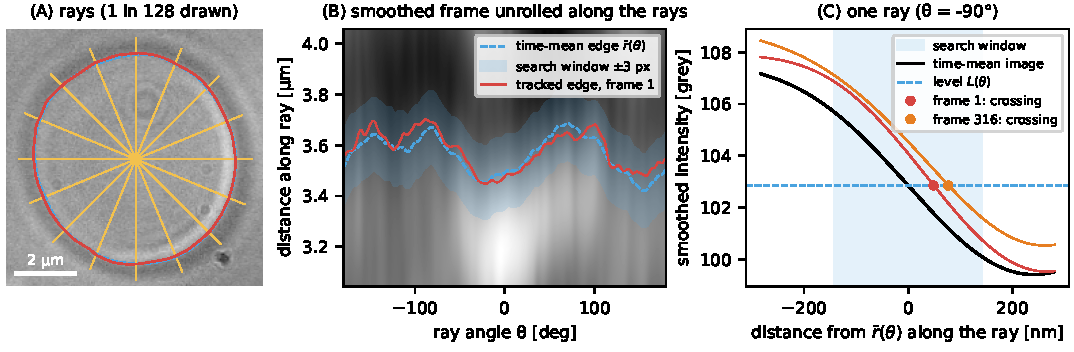
\includegraphics[width=\textwidth]{fig_contour}
\caption{Contour identification (free RBC~1). (A) Rays from the cell centre (1 in 128 of the 2048
drawn), the time-mean edge $\bar r(\theta)$ (blue, dashed) and the contour tracked in frame~1 (red).
(B) Frame~1, smoothed ($\sigma = 3$~px) and unrolled along the rays. The edge is searched only
within $\pm3$~px of $\bar r(\theta)$ (shaded). (C) Intensity along one ray: the time-mean image
(black) sets the ray's level $L(\theta)$ at $\bar r(\theta)$. In each frame the edge is the crossing
of that level (dots), here 28~nm further out in frame 316 than in frame~1.}
\label{fig:contour}
\end{figure*}

\subsection{Validation on synthetic frames}\label{sec:valid}
Real video has no ground truth, so we rendered synthetic frames from each video's own radial
intensity profile and its measured, spatially correlated pixel noise. On static synthetic frames
the per-ray noise floor was 8.3--20.2~nm. On moving synthetic membranes of four cells the tracker
recovered 95.8--96.5\% of the imposed motion, a gain of 0.96. Projected onto the contour modes, the
noise-only spectrum was 0.3--2.9~nm$^2$ per mode for modes 2--30, against $10^2$--$10^3$~nm$^2$ of
signal in the modes used for fitting. A gradient-peak tracker, with a floor of 29--59~nm, was
discarded at this step.

\subsection{Noise calibration}
Tracking noise $\zeta$ is white in time, so it adds a constant $2s_\zeta^2$ to the mean squared
displacement (MSD) at every lag. A video alone bounds it:
$s_\zeta \le s_{\zeta,\max} = \sqrt{\mathrm{MSD}(1~\text{ms})/2} = 9$--15~nm, the level at which
all of the 1~ms MSD would be noise. The static-synthetic floor exceeded this bound in 5 of 11
videos, so it is an upper bound rather than an estimate. An independent calibration came from 25
dust particles stuck to the glass, whose edge noise was 3.7--23.6~nm.

\subsection{Feature extraction: contour modes}
The tracked radius $r(\theta,t)$ is decomposed into Fourier modes,
$r(\theta,t) = R_0(t) + \sum_{|q|\ge2} h_q(t)\,e^{iq\theta}$, with $R_0$ fixing the enclosed area
and $q = \pm1$ (translation) removed. Each $h_q(t)$ is a 5000-sample complex time series. Modes
$q = 2$--6 carry 56--71\% of the noise-corrected shape variance and are the features the models are
fitted to.

\begin{figure}[t]
\centering
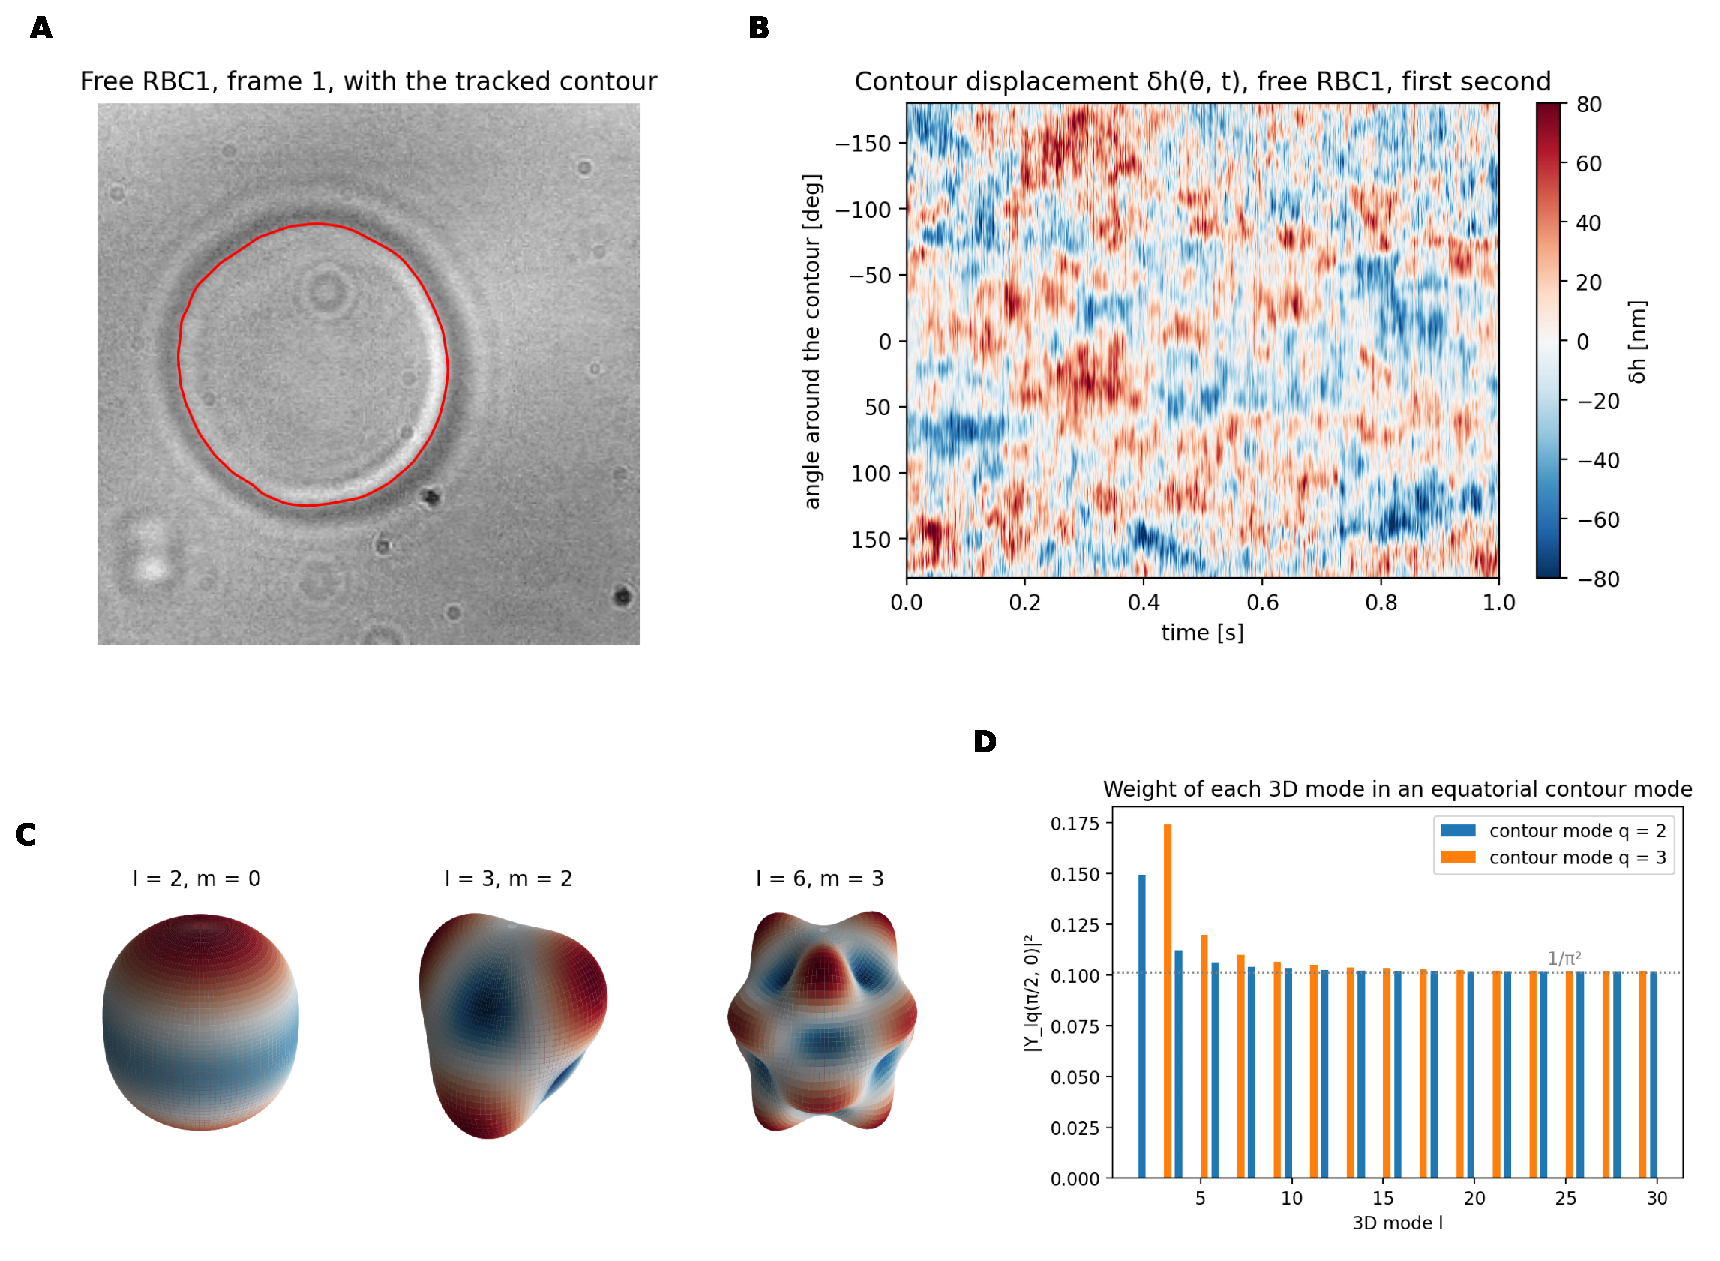
\includegraphics[width=\linewidth]{fig1_data_model}
\caption{Data and model. (A) A bright-field frame of free RBC~1 with the tracked contour. (B) Contour
displacement $\delta h(\theta,t)$ over the first second (red outward, blue inward). (C)
Spherical-harmonic shape modes, exaggerated. (D) Weight $|Y_{lq}(\tfrac\pi2,0)|^2$ of each 3D mode
$l$ in contour modes $q = 2$ and 3. The weights tend to $1/\pi^2$, so every contour mode mixes many
relaxation rates.}
\label{fig:data}
\end{figure}

% =================================================================================================
\section{Generative Model}\label{sec:model}

\subsection{Membrane dynamics}
We write the cell as a perturbed sphere,
$r(\vartheta,\varphi,t) = R[1 + \sum_{l\ge2}\sum_{m}\alpha_{lm}(t)Y_{lm}(\vartheta,\varphi)]$, with
complex spherical harmonics $Y_{lm}$. Each shape mode obeys an overdamped force balance between the
Helfrich bending and tension forces, viscous drag, thermal noise and a forcing
$f_{lm}$~\cite{milner1987}:
\begin{equation}
\dd\alpha_{lm} = -r_l\,\alpha_{lm}\,\dd t + f_{lm}\,\dd t + \sqrt{2D_l}\,\dd W_{lm},
\label{eq:mode}
\end{equation}
\begin{equation}
r_l = \frac{\kappa E_l\,l(l+1)}{\eta R^3(4l^3+6l^2-1)},\quad D_l = \frac{r_l k_BT}{\kappa E_l},
\label{eq:rates}
\end{equation}
with $E_l = (l-1)(l+2)[l(l+1)+\bar\sigma] + \bar\gamma$. Here $\kappa$ is the bending modulus,
$\bar\sigma = \sigma R^2/\kappa$ the reduced tension, $\bar\gamma = \gamma R^4/\kappa$ a reduced
confinement that stands in for the spectrin cytoskeleton, $\eta$ an effective viscosity and
$T = 310.15$~K. The rate $r_l$ is the Milner--Safran rate~\cite{milner1987}, and matches eq.~2
of~\cite{faizi2020} when $\bar\gamma = 0$. With an inner/outer viscosity contrast of about 10, as
measured for RBCs~\cite{john2025}, the denominator grows by a factor of 4.76 at $l = 2$ and 5.49 at
$l = 10$~\cite{faizi2020}. That divides the rates by the same factors, which is why the fitted
$\eta$ is an effective viscosity.

\textbf{Passive model P:} $f_{lm} \equiv 0$, so each mode is an Ornstein--Uhlenbeck (OU) process
with variance $k_BT/(\kappa E_l)$. \textbf{Active model A:} $f_{lm}$ is itself an OU process with
memory time $\tau_a$ and intensity $a$ times the thermal one, which gives each mode the spectrum
\begin{equation}
S_l(\omega) = \frac{2D_l\,[1 + a/(1+\omega^2\tau_a^2)]}{\omega^2 + r_l^2}.
\label{eq:spectrum}
\end{equation}
$(a,\tau_a)$ is shared by all modes, so A is a \emph{colored effective temperature}; as
$\tau_a \to 0$ the mode simply looks hotter, at $(1+a)T$. The label ``active'' says what A is meant
to represent. Nothing in A, or in contour data alone, shows that the forcing is ATP-driven. Model
A2 adds a second colored term. A has six parameters ($\kappa/k_BT$, $\bar\sigma$, $\bar\gamma$,
$\eta$, $a$, $\tau_a$) plus the noise level.

\subsection{Observation model}
The camera sees only the equatorial contour. A contour mode sums every 3D mode with the same
azimuthal number~\cite{milner1987,faizi2020},
\begin{equation}
h_q(t) = R\sum_{l\ge q,\ l+q\ \mathrm{even}} Y_{lq}(\tfrac\pi2,0)\,\alpha_{lq}(t),
\label{eq:proj}
\end{equation}
truncated at $l_{\max} = 40$. Even a passive membrane therefore puts many relaxation rates into
each contour mode (Fig.~\ref{fig:data}D). Each frame also averages the motion over the 1~ms
exposure, the tracker smooths along the contour (a gain per mode), and white localization noise is
added. To first order, exposure averaging makes each sampled $\alpha_{lq}$ an ARMA(1,1) process
with autoregressive root $e^{-r_l\Delta}$, $\Delta = 1$~ms. The observed spectrum, aliasing
included, is therefore the sum of these rational spectra plus a constant, and we compute it exactly.

% =================================================================================================
\section{Analysis and Evaluation Methods}\label{sec:analysis}

\subsection{Spectral likelihood}
P and A were fitted per video to modes $q = 2$--6 by the Whittle likelihood~\cite{whittle1953},
which treats periodogram ordinates as independent exponentials around the model spectrum. It suits
stationary Gaussian series whose spectrum is known in closed form, as it is here.

\subsection{Identifiability}
Each parameter was profiled with all the others re-optimized~\cite{raue2009}. A parameter counts as
practically identifiable when its 95\% profile interval is bounded. When a profile point fell below
the reported optimum, the fit was restarted from that point and every profile recomputed.

\subsection{Neural posterior estimation (NPE)}
As a check that does not depend on the Whittle frequency weighting, we trained a neural spline flow
on a band-pooled summary of binned periodograms by truncated sequential NPE~\cite{deistler2022},
with three rounds of $3\times10^4$ simulations from the same generative model, and applied it to
all 11 videos.

\subsection{Calibrated model selection}
P was compared with A by $\Delta\mathrm{AIC} = \mathrm{AIC}(P) - \mathrm{AIC}(A)$~\cite{akaike1974}.
With $\sim2.5\times10^4$ periodogram ordinates per video, any misspecified model can lose by a large
margin. We therefore calibrated $\Delta$AIC by a parametric bootstrap. Three passive generators
were fitted to four cells: P itself, P with a viscosity contrast of 10, and P with a log-normal
spread of each mode's rate. Each was simulated through the full observation model (20 replicates per
cell and generator) and refitted exactly as the data.

\subsection{Goodness of fit and surrogate tests}
Model A was checked against simulations at its estimate with a $\chi^2$ statistic on the spectral
summary. Non-Gaussianity (per-site and per-mode kurtosis) was tested against multivariate
phase-randomized surrogates~\cite{prichard1994}, which keep each site's spectrum and all
cross-spectra but destroy higher-order structure.

\subsection{Injection tests of the published markers}
To ask whether the published kickers are detectable at all, we rendered synthetic kicks of 100~nm,
lasting $\tau_0 \in \{20, 200\}$~ms at rates $\nu \in \{0.5, 2\}$~s$^{-1}$, into the real frames of
free RBC~1 at six sites. Their lateral standard deviation ran from 50 to 400~nm, with three seeds
each. The frames were then tracked with the same tracker. Short-time MSD exponents were refitted
after subtracting the calibrated noise, capped at $s_{\zeta,\max}$.

% =================================================================================================
\section{Results}\label{sec:results}

\subsection{Stiffness and temperature are not separately identifiable}
If all the noise is lumped into an effective temperature $T_\text{eff}$, the law of every mode in
(\ref{eq:mode})--(\ref{eq:proj}) depends only on $\kappa/k_BT_\text{eff}$, $\kappa/\eta$,
$\bar\sigma$ and $\bar\gamma$. It is therefore unchanged under
$(\kappa,\sigma,\gamma,\eta,T_\text{eff}) \mapsto c\,(\kappa,\sigma,\gamma,\eta,T_\text{eff})$ for
every $c > 0$: the modes are Gaussian OU processes, the rate depends on $\kappa/\eta$, the variance
on $k_BT_\text{eff}/\kappa$, and both ratios are scale-invariant. No modulus can be measured in
absolute units from fluctuations alone. The projection~(\ref{eq:proj}) nonetheless recovers the
\emph{ratios}. As a function of $\omega^2$, the spectrum of one contour mode is a sum of Lorentzians
$c_l/(\omega^2 + r_l^2)$ plus a noise constant. The sum is meromorphic, so its values on any
frequency interval determine every pole $\omega^2 = -r_l^2$ and its residue. Provided the rates are
distinct and increase with $l$ (which fails only when confinement dominates), three
distinct rates fix $\kappa/\eta$, $\bar\sigma$ and $\bar\gamma$ through $E_l$, whatever the
smoothing gain. On simulated data observed like the real data, the profile likelihood of $\kappa$
varied by less than $10^{-9}$ over $\pm0.4$ in $\log\kappa$ when $T_\text{eff}$ was free
(Fig.~\ref{fig:ident}), and the ratios were recovered within 4\%.

This matters for the published stiffening. The paired variance ratio free/trapped was 1.40, 1.64,
1.08 and 1.12 for RBC~1, 2, 10 and 13. If the two noise levels of a pair vary independently within
their bounds, the ranges are 1.07--1.69, 1.27--2.01, 0.91--1.29 and 0.73--1.76, so RBC~10 and 13
could lie below 1. Either way, a lower variance under the trap cannot be attributed to a stiffer
membrane rather than to weaker forcing.

\begin{figure}[t]
\centering
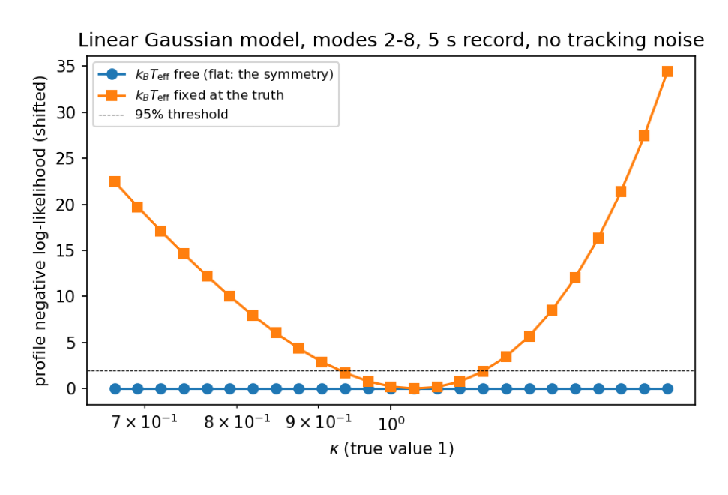
\includegraphics[width=0.85\linewidth]{fig3_identifiability}
\caption{Profile likelihood of the bending modulus $\kappa$ on simulated data (modes 2--8, 5~s).
With the effective temperature free (flat, to $10^{-9}$) $\kappa$ is unidentifiable; fixed at its
true value, it is identified.}
\label{fig:ident}
\end{figure}

\subsection{Four published markers are not supported by the imaging chain}
\emph{Spectral shape.} Caselli et al.\ fitted a sum of passive Milner--Safran modes plus one active
Lorentzian to the averaged spectrum (their Eq.~2), which we did not refit. We tested the narrower
per-mode reading. One Lorentzian per contour mode is the passive signature only without
projection. On synthetic \emph{passive} projected data, a single-Lorentzian test called 70--100\% of
mode components ``colored'', whereas the joint projected fit preferred P in 3 of 4 replicates
($\Delta$AIC $-3.3$, $-2.2$, $-3.7$, $+1.4$). A per-mode test therefore labels passive membranes
active.

\emph{Kickers.} Caselli et al.\ report kicks of about 100~nm at sites of lateral size up to about
100~nm~\cite{caselli2024}. Injected kicks of lateral width 50~nm (true per-site kurtosis 3.24--5.15)
were tracked at 2.87--3.05, inside the Gaussian-surrogate band in all 12 runs. At 100~nm they were
detected in only 4 of 12 runs; at 150~nm and wider they were detected (Fig.~\ref{fig:markers}A). The
reported kickers are therefore at or below the detection limit of the chain. On the real data,
per-site kurtosis lay inside the surrogate band in every video, and pooled kurtosis was 3.01--3.39
per cell, not the reported 4.1~\cite{caselli2024}.

\emph{Short-time exponent.} The reported sub-diffusive MSD exponent
$\alpha_\text{free} \approx 1/4$~\cite{caselli2024} can be manufactured by noise: an OU process with
true short-time exponent 1, plus white noise of the measured size, is fitted at $\alpha = 0.23$.
After subtracting the calibrated noise, the exponent was 0.29--0.81 in seven cells, and in the
other four it was set by the noise cap rather than the data (Fig.~\ref{fig:markers}B,C).

\emph{Diffusivity maps.} The published local ``diffusivity'' is a linear MSD slope over
$\tau < 20$~ms. For a stationary site $\mathrm{MSD}(\tau) = 2\sigma^2(1-\rho(\tau))$, so the slope
is the local variance $\sigma^2$ times a functional of the correlation $\rho$, and its reported correlation with that variance is
partly algebraic. That correlation (0.74 trapped above 0.49 free) was not reproduced per site:
pooled over the four pairs it was 0.15 trapped and 0.75 free.

\begin{figure*}[t]
\centering
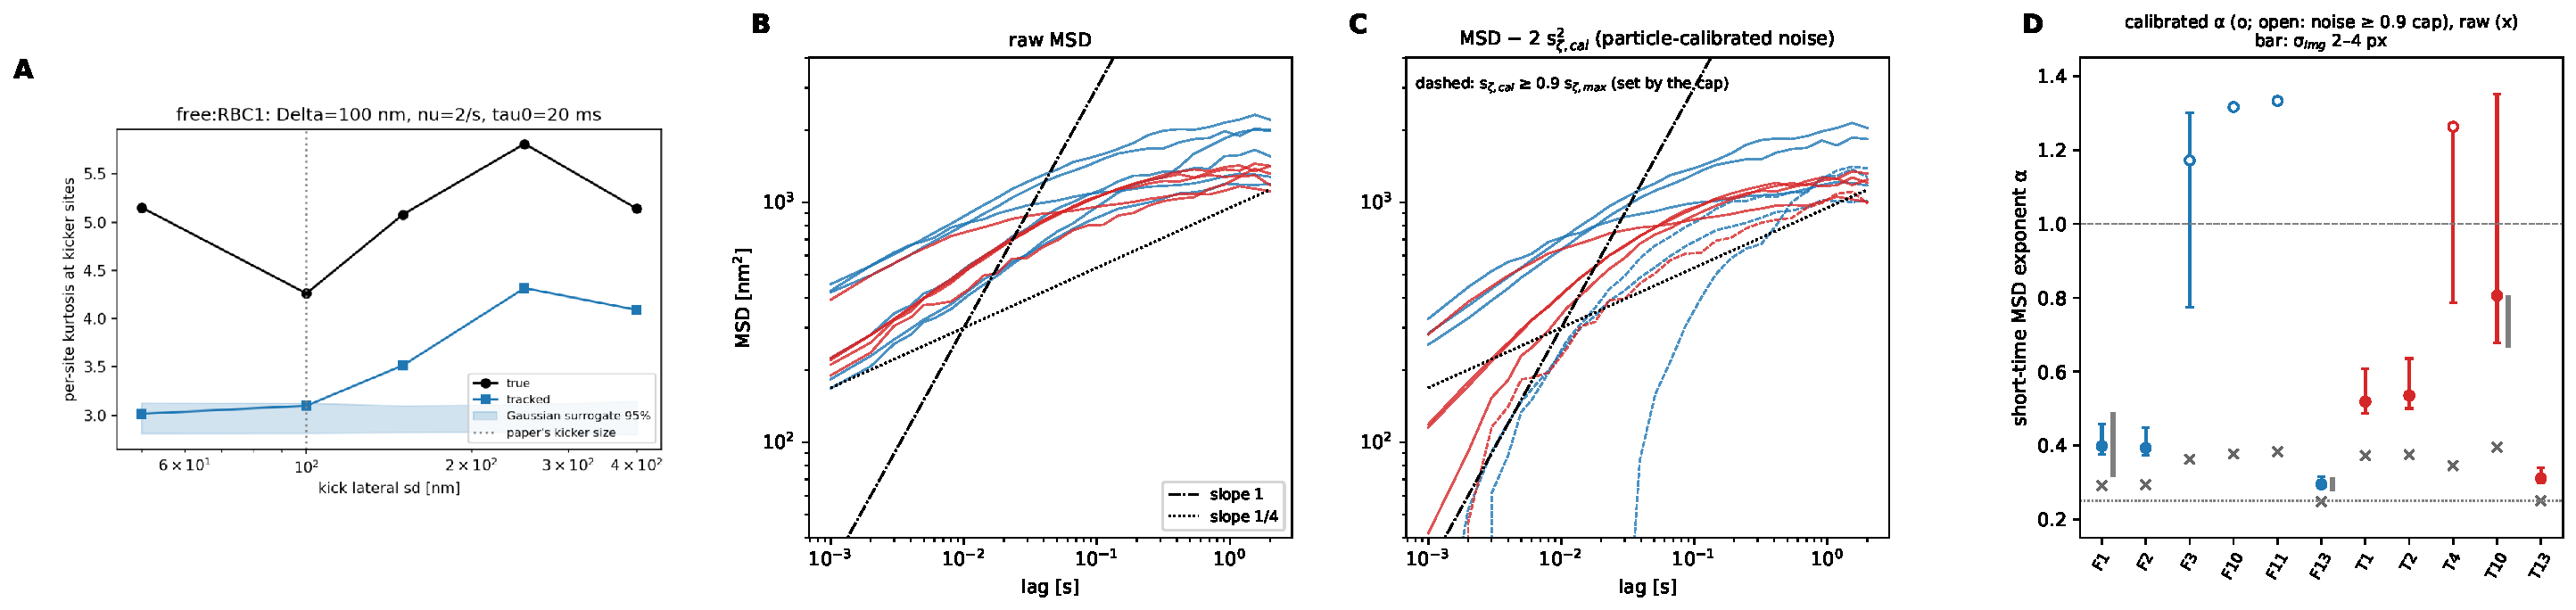
\includegraphics[width=0.9\textwidth]{fig4_markers}
\caption{Published markers through the imaging chain. (A) Per-site kurtosis at injected kicker
sites, true (black) and tracked (blue), against the lateral width of the kick, with the 95\%
Gaussian-surrogate band (free RBC~1, $\tau_0 = 20$~ms, $\nu = 2$~s$^{-1}$). (B) Site-averaged MSD
of every video (blue free, red trapped) with reference slopes 1 and 1/4. (C) The same after
removing white noise of $0.75\,s_{\zeta,\max}$, one of the scanned levels.}
\label{fig:markers}
\end{figure*}

\subsection{The passive model is rejected, but the active model misfits}
P was rejected in all 11 videos, free and trapped alike, with $\Delta$AIC $= +796$ to $+1479$
(Fig.~\ref{fig:selection}A). Under the passive nulls, the 95\% quantile of $\Delta$AIC was 26.9
(P), 36.3 (viscosity contrast) and 554 (spread of rates). The four calibration cells gave
1151--1479, above every null replicate by at least 530. The colored component is not an artefact of
these misfits either: under the nulls, A's fitted $\tau_a$ fell in 20--45~ms only with
$a < 10$, against $a = 53$--3200 on the data.

Rejecting P does not prove activity. A passive model with a very broad spread of rates comes close to A,
and the comparison is not converged in the rate quadrature: it beats A in all four calibration cells
with 5 quadrature nodes and in two with 15, and with 31 it is within 21 and 71 AIC of A in those two, at an effective viscosity of 1.8--3.6~Pa\,s, one and a half to two
orders of magnitude above the passive fits. The deposit contains no ATP-depleted or fixed recording
that would separate the two. Particles stuck to the glass rule out stage drift and linear focus
coupling as the source of the colored component.

Model A, in turn, is not an exact description of any cell. Against simulations at its estimate, the
observed $\chi^2$ was 488--900, where 99\% of simulations fall below 199--217. The data exceed A
below 2~Hz (median ratio 2.0) and fall below it at 3--30~Hz (0.53--0.93), and agree above 100~Hz
(Fig.~\ref{fig:selection}B). A second colored term (A2) was preferred in every cell ($\Delta$AIC
$+120$ to $+516$, times of 4--12 and 58--138~ms), but cut $\chi^2$ only to 312--582. The forcing
needs a spread of time scales, and A's fitted values are best-fit values of a misspecified model.
Within A, the forcing parameters were identifiable in every cell ($a = 53$--3200,
$\tau_a = 12$--60~ms), but $\kappa$ had no closed interval in any cell. The NPE agreed with the
profile likelihood on \emph{which} parameters are identifiable (91--100\% of cells per parameter),
but not on their values. Mode kurtosis lay inside its Gaussian null in all 11 videos, and a
softening drift of the slowest mode ($\theta_K \ge 0.5$) was excluded in all 8 testable videos.

\begin{figure*}[t]
\centering
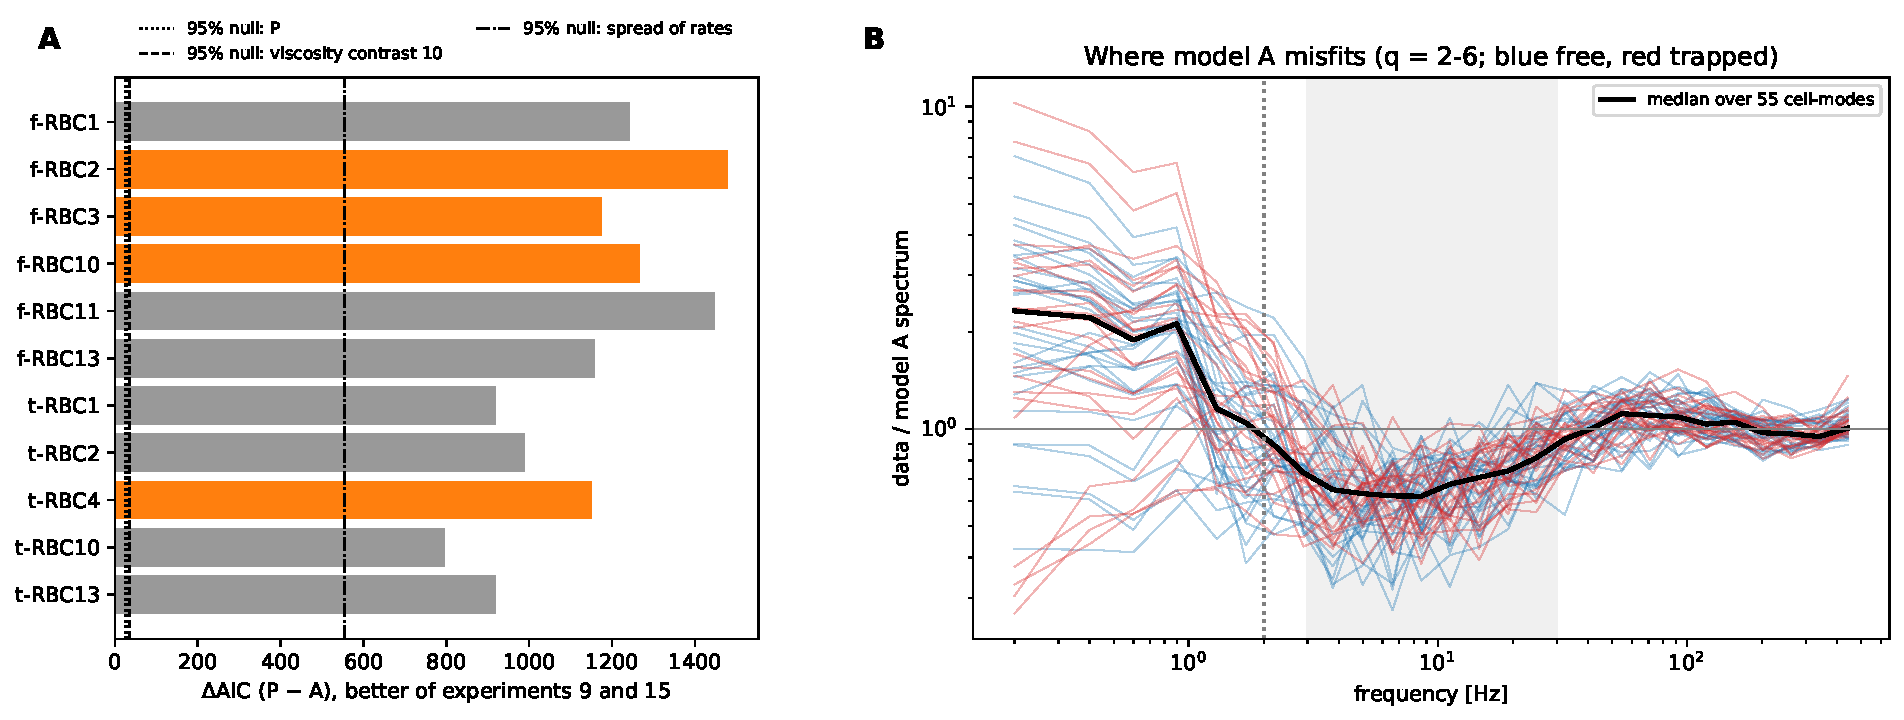
\includegraphics[width=0.9\textwidth]{fig5_model_selection}
\caption{Model evaluation. (A) $\Delta$AIC of passive P against active A for every video (f = free,
t = trapped), with the 95\% quantiles of $\Delta$AIC under three passive null generators (orange).
(B) Ratio of the data spectrum to model A for modes $q = 2$--6 of every video (blue free, red
trapped) and their median; the shading marks 3--30~Hz, where A overshoots.}
\label{fig:selection}
\end{figure*}

\subsection{The contour is low-dimensional; the model is not}
Ten mode pairs ($q = 2$--11) carried 90\% of the noise-corrected shape signal, and 12--16 carried
95\%. Free and trapped cells needed the same number, so trapping lowers the amplitude, not the
dimension. The fitted model does not truncate to a few equations, though. Coming within 1 nat of
the $l_{\max} = 40$ likelihood needed $l_{\max} = 26$--40 in 10 of 11 videos.

% =================================================================================================
\section{Using the Mined Model: Transport Inside the Cell}\label{sec:transport}

\subsection{Simulation set-up}
In the equatorial section $\Omega_t$ of the cell, the concentration $c$ of a signaling molecule
solves
\begin{equation}
\partial_t c + \nabla\cdot(\mathbf v c) = D\Delta c\ \ \text{in }\Omega_t,\qquad
D\,\partial_n c = J\chi\ \ \text{on }\partial\Omega_t,
\label{eq:interior}
\end{equation}
starting from $c = 0$, with molecules entering at rate $J$ through one channel of profile $\chi$.
The cytosol is incompressible and enclosed, so the moving wall drags it along. Its velocity
$\mathbf v$ is the no-slip Stokes flow, fixed by the wall path alone. For a wall mode
$\alpha_n\cos n\varphi$ its stream function is
$\psi = R\,g_n(r/R)\,\dot\alpha_n\sin n\varphi$ with
$g_n(\rho) = [(n+1)\rho^n + (1-n)\rho^{n+2}]/(2n)$, read in the Stratonovich sense for a rough
wall~\cite{kunita1990}. For comparison we also solved a still medium ($\mathbf v \equiv 0$), in
which the wall sweeps molecules. The output is the share of injected mass within $0.3R$ of the
centre at $T = 0.05R^2/D$,
\begin{equation}
\Phi = \frac{1}{JT}\int_{|x|<0.3R} c(x,T)\,\dd x,
\label{eq:phi}
\end{equation}
for $D = 5$ and $0.5~\mu$m$^2$/s. Walls came from model A refitted to each of the 11 cells (12
paths per cell) and, separately, from the tracked contours themselves (modes $q = 2$--6). Every
comparison used common random numbers. The wall-motion effect was estimated antithetically, as the
mean over a wall $h$ and its reflection $-h$, each against the same wall frozen at its initial
shape. Equation~(\ref{eq:interior}) was solved by a positivity-preserving finite-volume scheme on
comoving coordinates~\cite{lepotier2005,yuan2008}, with an exactly incompressible discrete flow.
Results were extrapolated from grids of 24 and 48 radial cells and checked against Brownian-particle
references.

\subsection{Prediction before computation}
With the cytosol carried, a fluid parcel follows the wall back and forth rather than drifting. Its
displacement is bounded in mean square for a stationary wall, so wall motion should act only through
the wall's variance. A scaling argument gives
\[
\frac{\Delta\Phi}{\Phi} \sim \frac{\mathrm{var}(h)}{DT} = 20\Big(\frac{\sigma_{\delta h}}{R}\Big)^2
\approx 0.07\text{--}0.13\%
\]
for the model walls ($\sigma_{\delta h}/R = 0.006$--0.008). This is a heuristic, not a theorem. It
would take $\sigma_{\delta h} \approx 90$~nm for a 1\% effect and 280~nm for 10\%.

\subsection{Results}
Table~\ref{tab:transport} gives the pooled changes. With the cytosol carried, the antithetic
wall-motion effect after grid extrapolation was $-0.03 \pm 0.01\%$ ($D = 5$) and $-0.02 \pm 0.01\%$
($D = 0.5$) of $\Phi$, within $\pm0.11\%$ in every cell. On the coarse grid alone the same contrast appeared
as $+0.38$ and $+0.62\%$, so most of the apparent effect was discretization error. To resolve the
effect without a grid, we ran particles on the walls of free RBC~1 scaled by a factor $s$
(Fig.~\ref{fig:motion}A). The antithetic effect followed $bs^2 + cs^4$, fitted at $s = 2.5$, 5 and
10, and a held-out run at $s = 1$ agreed with $b + c$ within one standard error in 5 of 6 cases.
Over 12 walls, $b = -0.14 \pm 0.06\%$ of $\Phi$ (Fig.~\ref{fig:motion}B). The effect is quadratic in the amplitude and of the
size predicted above.

Walls taken directly from the videos, which do not rely on the misfitting model A, gave the same
answer (Fig.~\ref{fig:motion}C): $-0.03\pm0.02\%$ ($D = 5$) and $-0.03\pm0.03\%$ ($D = 0.5$). For
their amplitudes ($\sigma_{\delta h}/R = 0.0042$--0.0062) the estimate gives 0.04--0.08\%. The choice
of medium matters little once the grid is converged: carried minus still was $-0.2$ to $-0.6\%$
pooled (Table~\ref{tab:transport}). The particle references put the extrapolated grid within about
$\pm0.4$ points.

\begin{table}[t]
\centering
\caption{Change in $\Phi$ (\% of $\Phi$), pooled over 11 cells $\times$ 12 model-A wall paths;
coarse grid ($N_r = 24$) and extrapolated ($Q^\ast$). Mean $\pm$ standard error. $^\dagger$Antithetic.}
\label{tab:transport}
\footnotesize
\setlength{\tabcolsep}{3pt}
\resizebox{\linewidth}{!}{%
\begin{tabular}{lcccc}
\toprule
 & \multicolumn{2}{c}{$D = 5~\mu$m$^2$/s} & \multicolumn{2}{c}{$D = 0.5~\mu$m$^2$/s}\\
 & $N_r{=}24$ & $Q^\ast$ & $N_r{=}24$ & $Q^\ast$\\
\midrule
Medium: carried$-$still & $-1.60{\pm}0.21$ & $-0.22{\pm}0.21$ & $-2.83{\pm}0.14$ & $-0.56{\pm}0.13$\\
Motion, still medium & $+2.19{\pm}0.46$ & $+0.33{\pm}0.40$ & $+4.26{\pm}0.44$ & $+1.27{\pm}0.39$\\
Motion, carried$^\dagger$ & $+0.38{\pm}0.01$ & $-0.03{\pm}0.01$ & $+0.62{\pm}0.01$ & $-0.02{\pm}0.01$\\
\bottomrule
\end{tabular}}
\end{table}

\begin{figure*}[t]
\centering
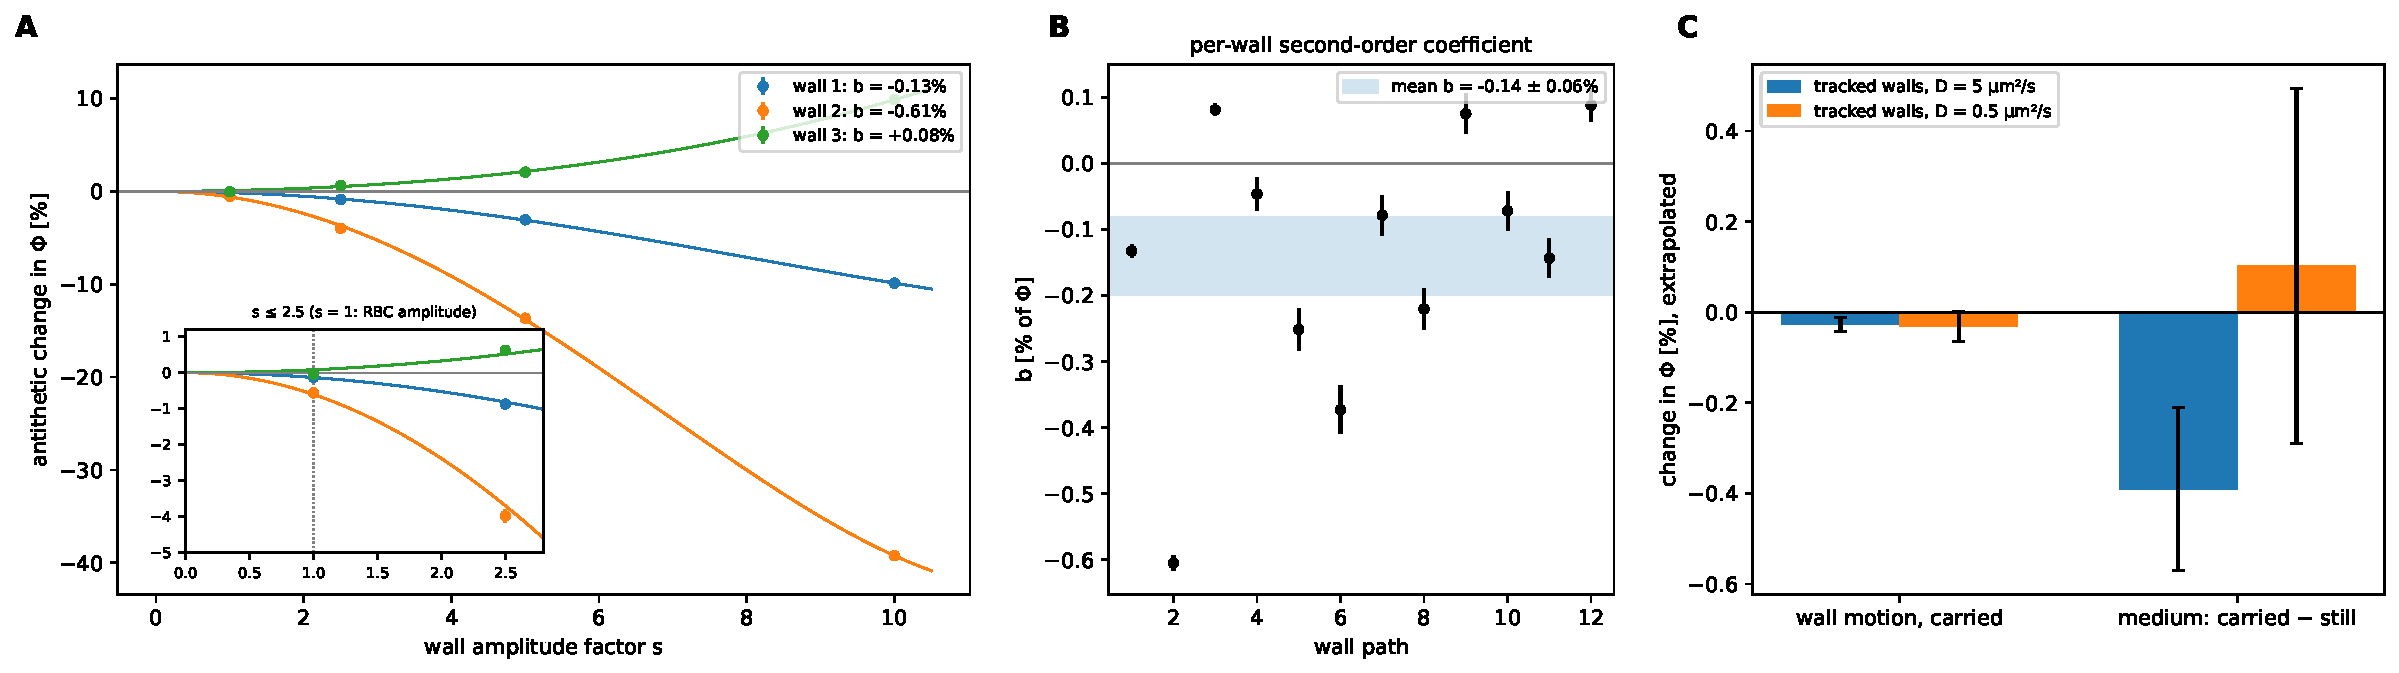
\includegraphics[width=0.9\textwidth]{fig6_wall_motion}
\caption{The wall-motion effect. (A) Particle simulations on the model-A walls of free RBC~1
($D = 5~\mu$m$^2$/s), scaled by an amplitude factor $s$. The antithetic effect follows
$bs^2 + cs^4$ (curves fitted to $s = 2.5$, 5, 10; $s = 1$ held out). (B) The fitted second-order
coefficient $b$ of each of the 12 walls ($\pm$ standard error) and their mean (band). (C) Walls taken from the
videos: extrapolated wall-motion effect with the cytosol carried, and the medium contrast, in \% of
$\Phi$, pooled over 11 videos (mean $\pm$ standard error).}
\label{fig:motion}
\end{figure*}

% =================================================================================================
\section{Discussion}\label{sec:discussion}

\textbf{What the data identify.} Flicker spectra determine ratios of the membrane moduli
($\kappa/\eta$, $\bar\sigma$, $\bar\gamma$) but not stiffness and effective temperature separately.
This is a structural property of the model, not a shortage of data, and no amount of the same kind
of recording removes it. The ``stiffening'' under the optical trap is therefore equally a fall in
forcing.

\textbf{What the data do not show.} Evaluation, not fitting, drove the conclusions. A naive per-mode
test, an uncalibrated $\Delta$AIC and an uncorrected MSD exponent would each have reported
``activity''. Injection tests, calibrated nulls and noise subtraction remove three published
markers, and the diffusivity-variance correlation is partly algebraic. What survives is a Gaussian,
colored component that a passive model with ordinary parameters cannot produce, but that has no
single time scale. Whether it is metabolic activity, or the misfit of a quasi-spherical model to a
biconcave cell, the data cannot say without an ATP-depleted or fixed control.

\textbf{What the model predicts.} At RBC amplitude, wall motion changes the mean transport by about
0.1\% or less, at second order in the amplitude, and the medium by about 1\% or less. A frozen wall
shape therefore predicts the mean over wall paths to that accuracy, but not a single path: freezing
the tracked wall at its time-mean shape misses the transport on one path by 3.3\% rms ($D =
5~\mu$m$^2$/s), and freezing it at a sampled shape by 4.5\%. The scaling $20(\sigma_{\delta h}/R)^2$ says where
the wall would matter: about 90~nm of motion for 1\% and 280~nm for 10\%. Red blood cells thus test
the method rather than show a large effect, and cells with larger excursions, such as blebs and
lamellipodia, are where it becomes quantitative. Two numerical lessons carry over to any
moving-boundary transport problem. A first-order remap of a moving wall converges to the wrong
diffusion coefficient. And a small transport contrast measured on one grid can be mostly
discretization error.

% =================================================================================================
\section{Limitations}\label{sec:limits}

Each stage of the pipeline rests on assumptions that bound what the conclusions can claim.

\textbf{Data.} The deposit holds 11 videos of seven cells from one laboratory, and the free--trapped
comparisons rest on four pairs. Each record lasts 5~s, so the spectrum is resolved only down to
0.2~Hz, which is near the band below 2~Hz where model A misfits most. There is no ATP-depleted,
fixed or temperature-varied control, so no part of the colored component can be attributed to
metabolism. All standard errors are conditional on these cells.

\textbf{Contour identification.} The camera sees one optical section, assumed to be the equator. The
level crossing~(\ref{eq:crossing}) follows an optical feature of the rim, not the membrane itself. A
change of focus or illumination moves that feature without moving the membrane. Particles stuck to
the glass rule out stage drift and linear focus coupling as the source of the colored component, but
not every optical artefact. The synthetic validation frames are drawn under the same assumption as
the tracker, that the rim pattern moves rigidly with the membrane. The gain and noise floors
therefore do not test that assumption. The tracking noise is bounded, not measured: the
static-synthetic floor exceeded the MSD bound in 5 of 11 videos. Rigid rotation is not removed.
Aligning each frame to the mean shape removes 4--30\% of the $q = 2$--6 variance, but this is an
upper bound, since only three videos show the common angle across modes that a rigid rotation
produces. The noise-corrected short-time MSD exponent depends on the image smoothing by more than
its calibration uncertainty.

\textbf{Model.} The membrane is a quasi-sphere, although the red cell is a biconcave disc. The
spectrin cytoskeleton enters only through the confinement term $\bar\gamma$, and one effective
viscosity absorbs the inner/outer contrast. Both models are linear and Gaussian. That suits these
data, whose mode kurtosis is Gaussian, but it excludes nonlinear drift and non-Gaussian forcing by
construction. Model A, with one forcing time, misfits every cell, and even the two-time model A2
leaves $\chi^2$ at 312--582. The fitted values are therefore best-fit parameters of misspecified
models, not physical constants. Stiffness and effective temperature are not separately identifiable
in principle, $\kappa$ is not identifiable within A, and the label ``active'' carries no evidence of
ATP use.

\textbf{Inference and evaluation.} The Whittle likelihood assumes stationary Gaussian series and
treats periodogram ordinates as independent, which holds only asymptotically: leakage couples
neighbouring frequencies, most of all at the low end of a 5~s record. A's likelihood has several
local optima. A later refit of free RBC~1 from 13 starting points found an optimum 43 log-likelihood
units better than the one used here ($\tau_a = 31$ rather than 27.5~ms, $a = 563$ rather than 935),
still inside the reported ranges. The $\Delta$AIC null was calibrated with three passive generators
on four cells (80 replicates per generator), so other forms of passive misspecification are untested.
The comparison with the broad-spread passive model is not converged in the rate quadrature. The NPE
agreed with the profile likelihood on which parameters are identifiable, but not on their values.

\textbf{Transport simulation.} Transport is computed in a 2D equatorial section of a 3D cell. The 2D
Stokes flow driven by the contour differs from the 3D flow of the same outline: the azimuthal wall
velocity is $2q/[l(l+1)]$ in 3D against $1/q$ in 2D, a third larger for $l = q = 2$. The walls carry
only modes $q = 2$--6 (56--71\% of the shape variance) and come from the misfitting model A, although
walls taken from the videos agree. Molecules are points with one diffusion coefficient. They do not
bind, crowd or cross the membrane, and they enter through one channel of fixed angular position.
There is one output, $\Phi$, at one time and one target radius. The second-order coefficient was
measured in one cell at one $D$ and is not proved. A red blood cell has no nucleus, so it stands in
for, rather than represents, the intracellular targets that motivate the question.

% =================================================================================================
\section{Conclusion}
A full data-mining pipeline (validated preprocessing, a physical generative model, calibrated
evaluation and simulation-based interpretation) turned 11 flicker videos into three answers. Contour
data identify ratios of the membrane moduli but not absolute stiffness. The published evidence for
localized active kicks does not survive the imaging chain, although a passive single-rate model is
also rejected. And at red-blood-cell amplitude the moving wall changes the mean interior transport
by only about 0.1\%, as a simple variance argument predicts, while single paths differ from a
frozen wall by a few per cent. All analyses are scripted and reproducible from
the project repository, \url{https://github.com/tlstellGSU/brownian_cells}.

\bibliographystyle{IEEEtran}
\bibliography{ieee_refs,ieee_extra}

\end{document}
